\documentclass[12pt, a4paper, hidelinks]{article}

\usepackage[icelandic]{babel}
\usepackage[T1]{fontenc}
\usepackage[utf8]{inputenc}


\usepackage{amsmath, amssymb, amsfonts}
\usepackage{mathtools}

\usepackage[outputdir=cache]{minted}
\usemintedstyle{default}
\renewcommand{\listingscaption}{Forrit}

\usepackage{url}
\usepackage{hyperref}
\usepackage[hang, flushmargin, bottom]{footmisc}

\usepackage[svgnames]{xcolor}
\usepackage{tabularx}
\usepackage{float}
\usepackage{graphicx}
\usepackage{booktabs}
\usepackage{enumerate}
\usepackage{multirow}
\usepackage{tikz}
\usetikzlibrary{arrows}
\usepackage{pifont}
\usepackage{multicol}
\usepackage{tcolorbox}
\usepackage{forest}

\usepackage{caption}
\usepackage{subcaption}

\newcommand{\cmark}{\color{Green}\ding{51}}
\newcommand{\xmark}{\color{Red}\ding{55}}

\usepackage{times, mathptmx}
\usepackage[scaled=0.85]{beramono}

\newenvironment{code}{\captionsetup{type=listing}}{}

\usepackage{fancyhdr}
\pagestyle{fancy}
\fancyhf{}
\fancyhead[L]{Kári Hlynsson}
\fancyhead[C]{TÖL203G Heimadæmi 9}
\fancyhead[R]{\today}
\fancyfoot[C]{\thepage}

\newcommand{\doctitle}{\uppercase{Heimadæmi 9}}
\newcommand{\coursename}{Tölvunarfræði 2}
\newcommand{\coursenum}{TÖL203G}

% ——— Mengjatákn
\newcommand{\N}{\mathbb{N}}
\newcommand{\Z}{\mathbb{Z}}
\newcommand{\Q}{\mathbb{Q}}
\newcommand{\R}{\mathbb{R}}
\newcommand{\C}{\mathbb{C}}

% ——— Vigrar
\renewcommand{\u}{\mathbf{u}}
\renewcommand{\v}{\mathbf{v}}
\renewcommand{\b}{\mathbf{b}}
\newcommand{\w}{\mathbf{w}}
\newcommand{\p}{\mathbf{p}}
\newcommand{\x}{\mathbf{x}}
\newcommand{\y}{\mathbf{y}}
\newcommand{\z}{\mathbf{z}}

% Define styles for nodes in the binary tree
\tikzset{
  binarytree/.style={
    draw,
    circle,
    thick,
    minimum size=0.75cm,
    inner sep=0pt,
    font=\sffamily\small
  },
  binaryedge/.style={
    draw,
    line width=1mm,
    red
  },
  binarytree empty/.style={
    draw=none,
    fill=none
  }
}

\graphicspath{{img}}

\begin{document}
\thispagestyle{plain}
\centerline{\bfseries\Large\doctitle}
\medskip
\centerline{\large\coursenum\ \coursename}
\bigskip

\centerline{\large Kári Hlynsson\footnote{Slóð á Github kóða: \url{https://github.com/lvthnn/TOL203G/tree/master/HD9}}}
\bigskip
\centerline{Háskóli Íslands}
\medskip
\centerline{\today}

\section*{Verkefni 1}
Tvö net eru einsmóta (\emph{isomorphic}) ef hægt er að endurnefna hnút annars netsins þannig að það sé nákvæmlega eins og hitt.\@ Teiknið upp öll möguleg einsmóta (óstefnd) einföld net með (a) tvo hnúta, (b) þrjá hnúta og (c) fjóra hnúta.

\subsection*{Lausn}
\subsubsection*{Hluti (a)}
\begin{figure}[H]
    \centering
    \begin{subfigure}[b]{0.45\textwidth}
        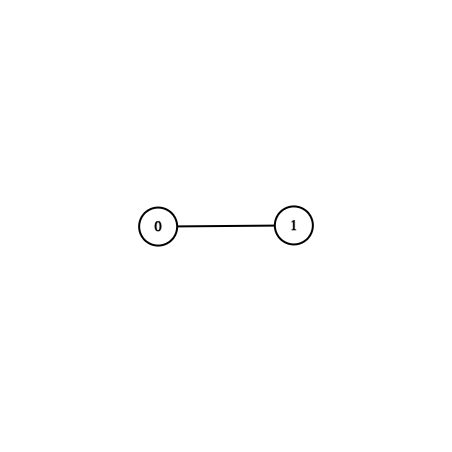
\includegraphics[width=\textwidth]{graph_v2_1.png}
    \end{subfigure}
    \begin{subfigure}[b]{0.45\textwidth}
        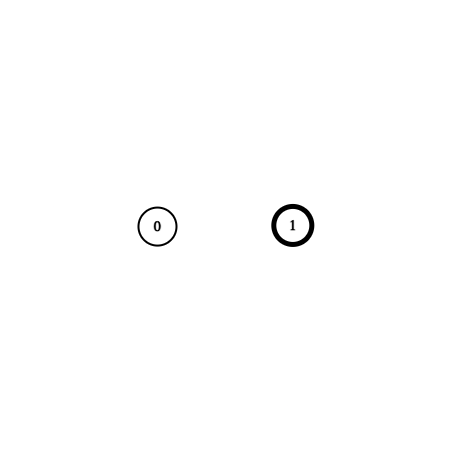
\includegraphics[width=\textwidth]{graph_v2_2.png}
    \end{subfigure}
    \caption{Einsmótanir fyrir net með $|V| = 2$}
    \label{fig:my_label}
\end{figure}

\subsubsection*{Hluti (b)}
\begin{figure}[H]
    \centering
    \begin{subfigure}[b]{0.45\textwidth}
        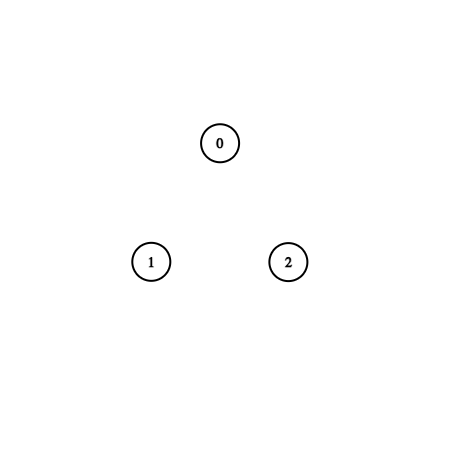
\includegraphics[width=\textwidth]{graph_v3_1.png}
    \end{subfigure}
    \begin{subfigure}[b]{0.45\textwidth}
        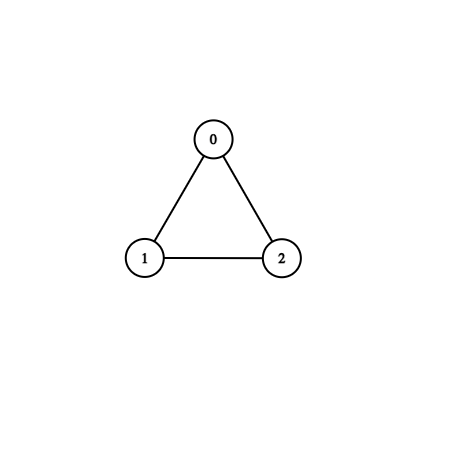
\includegraphics[width=\textwidth]{graph_v3_2.png}
    \end{subfigure}
\end{figure}
\begin{figure}[H]
    \centering
    \begin{subfigure}[b]{0.45\textwidth}
        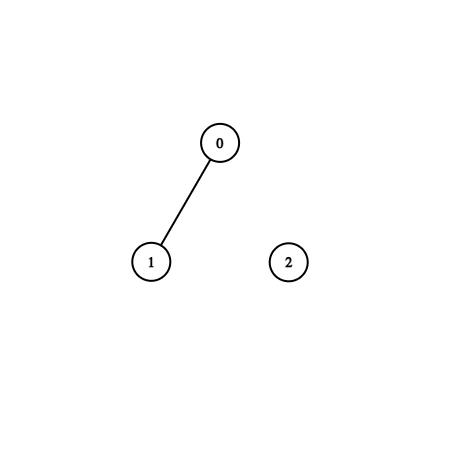
\includegraphics[width=\textwidth]{graph_v3_3.png}
    \end{subfigure}
    \begin{subfigure}[b]{0.45\textwidth}
        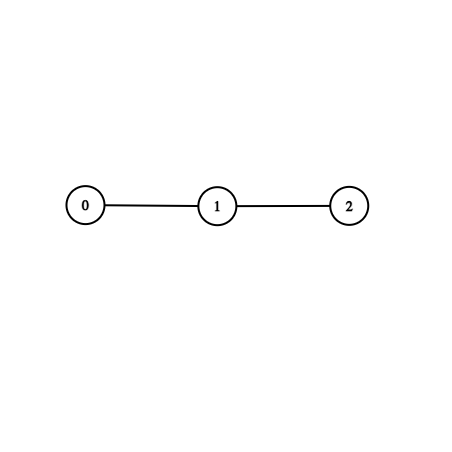
\includegraphics[width=\textwidth]{graph_v3_4.png}
    \end{subfigure}
    \caption{Einsmótanir fyrir net með $|V| = 3$}
\end{figure}

\newpage

\subsubsection*{Hluti (c)}
\begin{figure}[H]
    \centering
    \begin{subfigure}[b]{0.45\textwidth}
        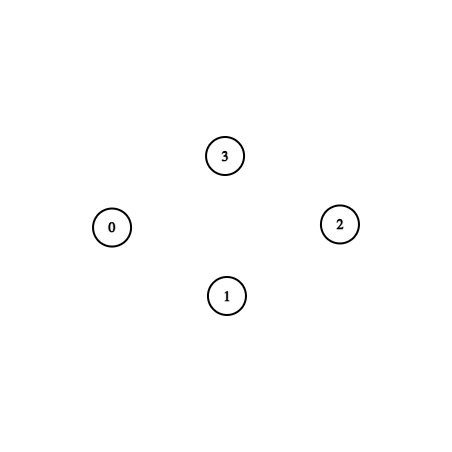
\includegraphics[width=\textwidth]{graph_v4_1.png}
    \end{subfigure}
    \begin{subfigure}[b]{0.45\textwidth}
        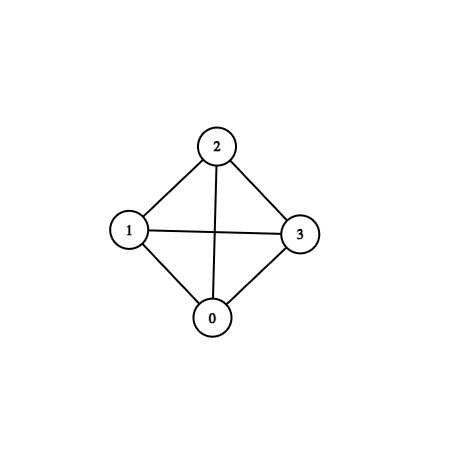
\includegraphics[width=\textwidth]{graph_v4_2.png}
    \end{subfigure}
\end{figure}
\begin{figure}[H]
    \centering
    \begin{subfigure}[b]{0.45\textwidth}
        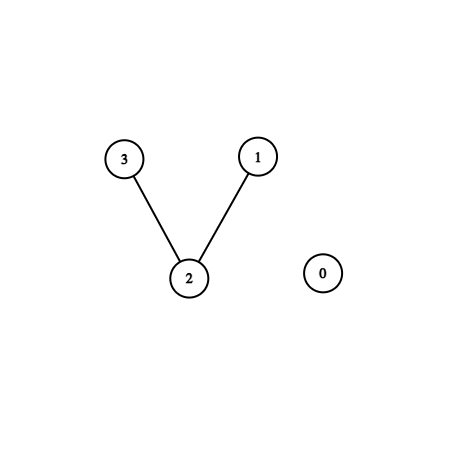
\includegraphics[width=\textwidth]{graph_v4_3.png}
    \end{subfigure}
    \begin{subfigure}[b]{0.45\textwidth}
        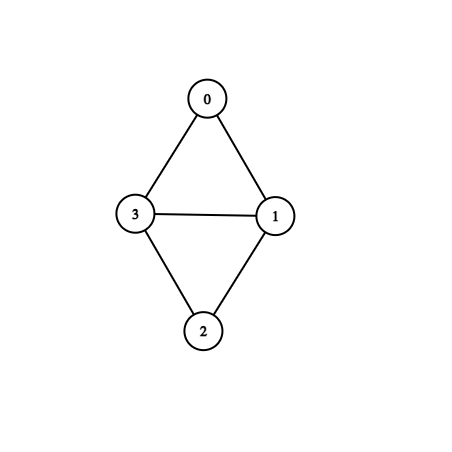
\includegraphics[width=\textwidth]{graph_v4_4.png}
    \end{subfigure}
\end{figure}
\begin{figure}[H]
    \centering
    \begin{subfigure}[b]{0.45\textwidth}
        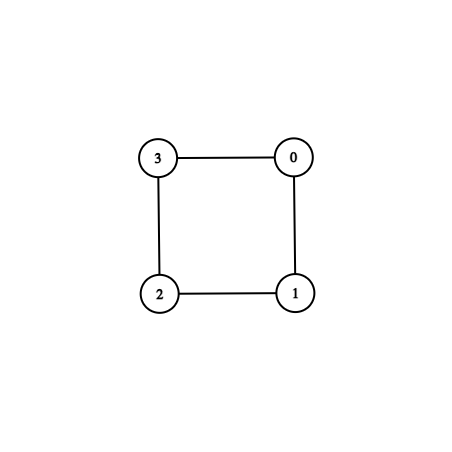
\includegraphics[width=\textwidth]{graph_v4_5.png}
    \end{subfigure}
    \begin{subfigure}[b]{0.45\textwidth}
        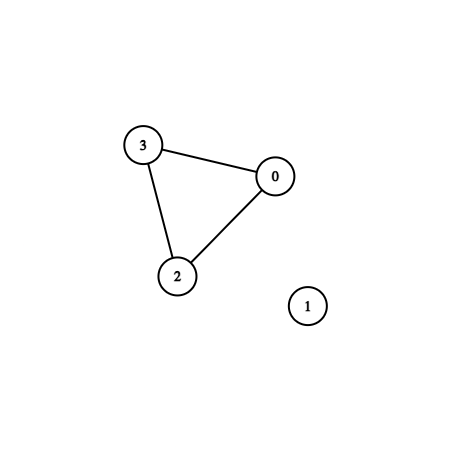
\includegraphics[width=\textwidth]{graph_v4_6.png}
    \end{subfigure}
\end{figure}
\begin{figure}[H]
    \centering
    \begin{subfigure}[b]{0.45\textwidth}
        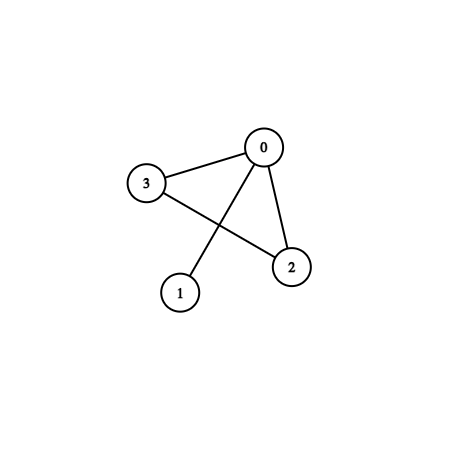
\includegraphics[width=\textwidth]{graph_v4_7.png}
    \end{subfigure}
    \begin{subfigure}[b]{0.45\textwidth}
        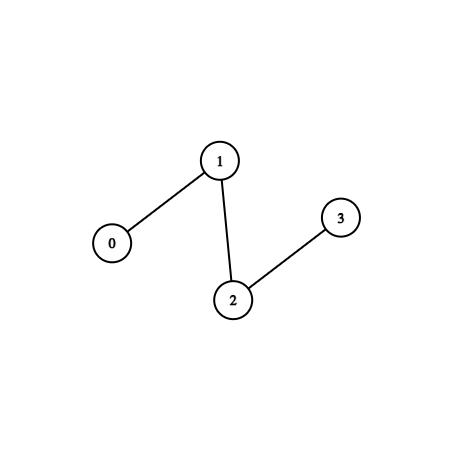
\includegraphics[width=\textwidth]{graph_v4_8.png}
    \end{subfigure}
\end{figure}
\begin{figure}[H]
    \centering
    \begin{subfigure}[b]{0.45\textwidth}
        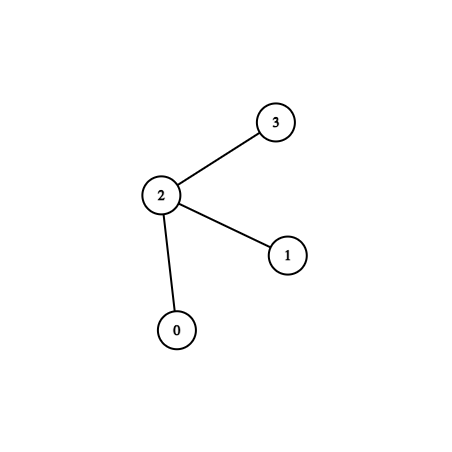
\includegraphics[width=\textwidth]{graph_v4_9.png}
    \end{subfigure}
    \begin{subfigure}[b]{0.45\textwidth}
        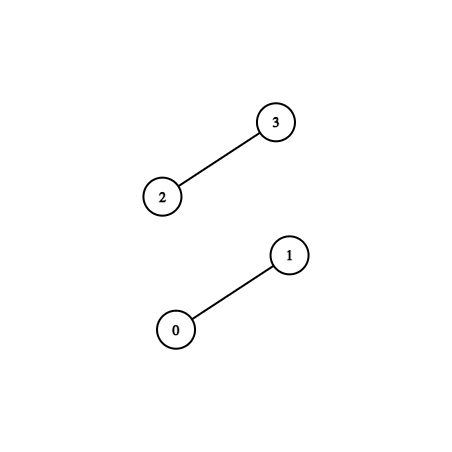
\includegraphics[width=\textwidth]{graph_v4_10.png}
    \end{subfigure}
\end{figure}
\begin{figure}[H]
    \centering
    \begin{subfigure}[b]{0.45\textwidth}
        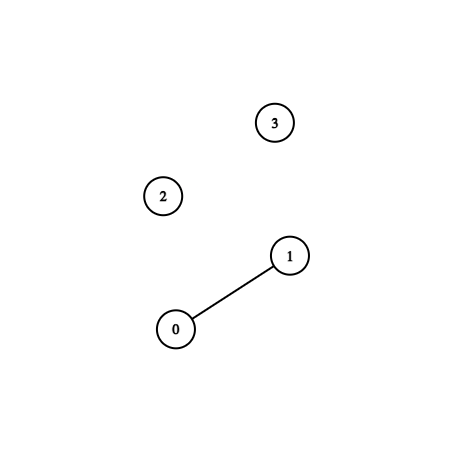
\includegraphics[width=\textwidth]{graph_v4_11.png}
    \end{subfigure}
    \caption{Einsmótanir fyrir net með $|V| = 4$}
\end{figure}

\newpage

\section*{Verkefni 2}
Dæmi 4.1.5 í kennslubók. Þið eigið að endurbæta aðferðina \texttt{addEdge} í klasanum \texttt{Graph}, þannig sjálflykkjur og samsíða leggir séu ekki leyfð. Kallið fram frábrigðið \texttt{IllegalArgumentException} ef reynt er að setja inn sjálflykkju eða samsíða legg. Skilið breyttu aðferðinni \texttt{addEdge} og skjáskoti af keyrslu \texttt{Graph} á skránni \texttt{nosimpG.txt}.
\subsection*{Lausn}
Nýja útfærslan á aðferðinni er sýnd fyrir neðan.
\begin{listing}[H]
\centering
\inputminted[linenos, fontsize=\small,breaklines, firstline=125, lastline=135]{java}{../src/V2/Graph.java} 
\end{listing}
\noindent
Í keyrslunni kemur upp \texttt{IllegalArgumentException} því við reynum að bæta við samsíða legg, sem ber saman við \texttt{nosimpG.txt}, eins og von var á. Sjá mynd á næstu síðu.
\begin{figure}[H]
\centering
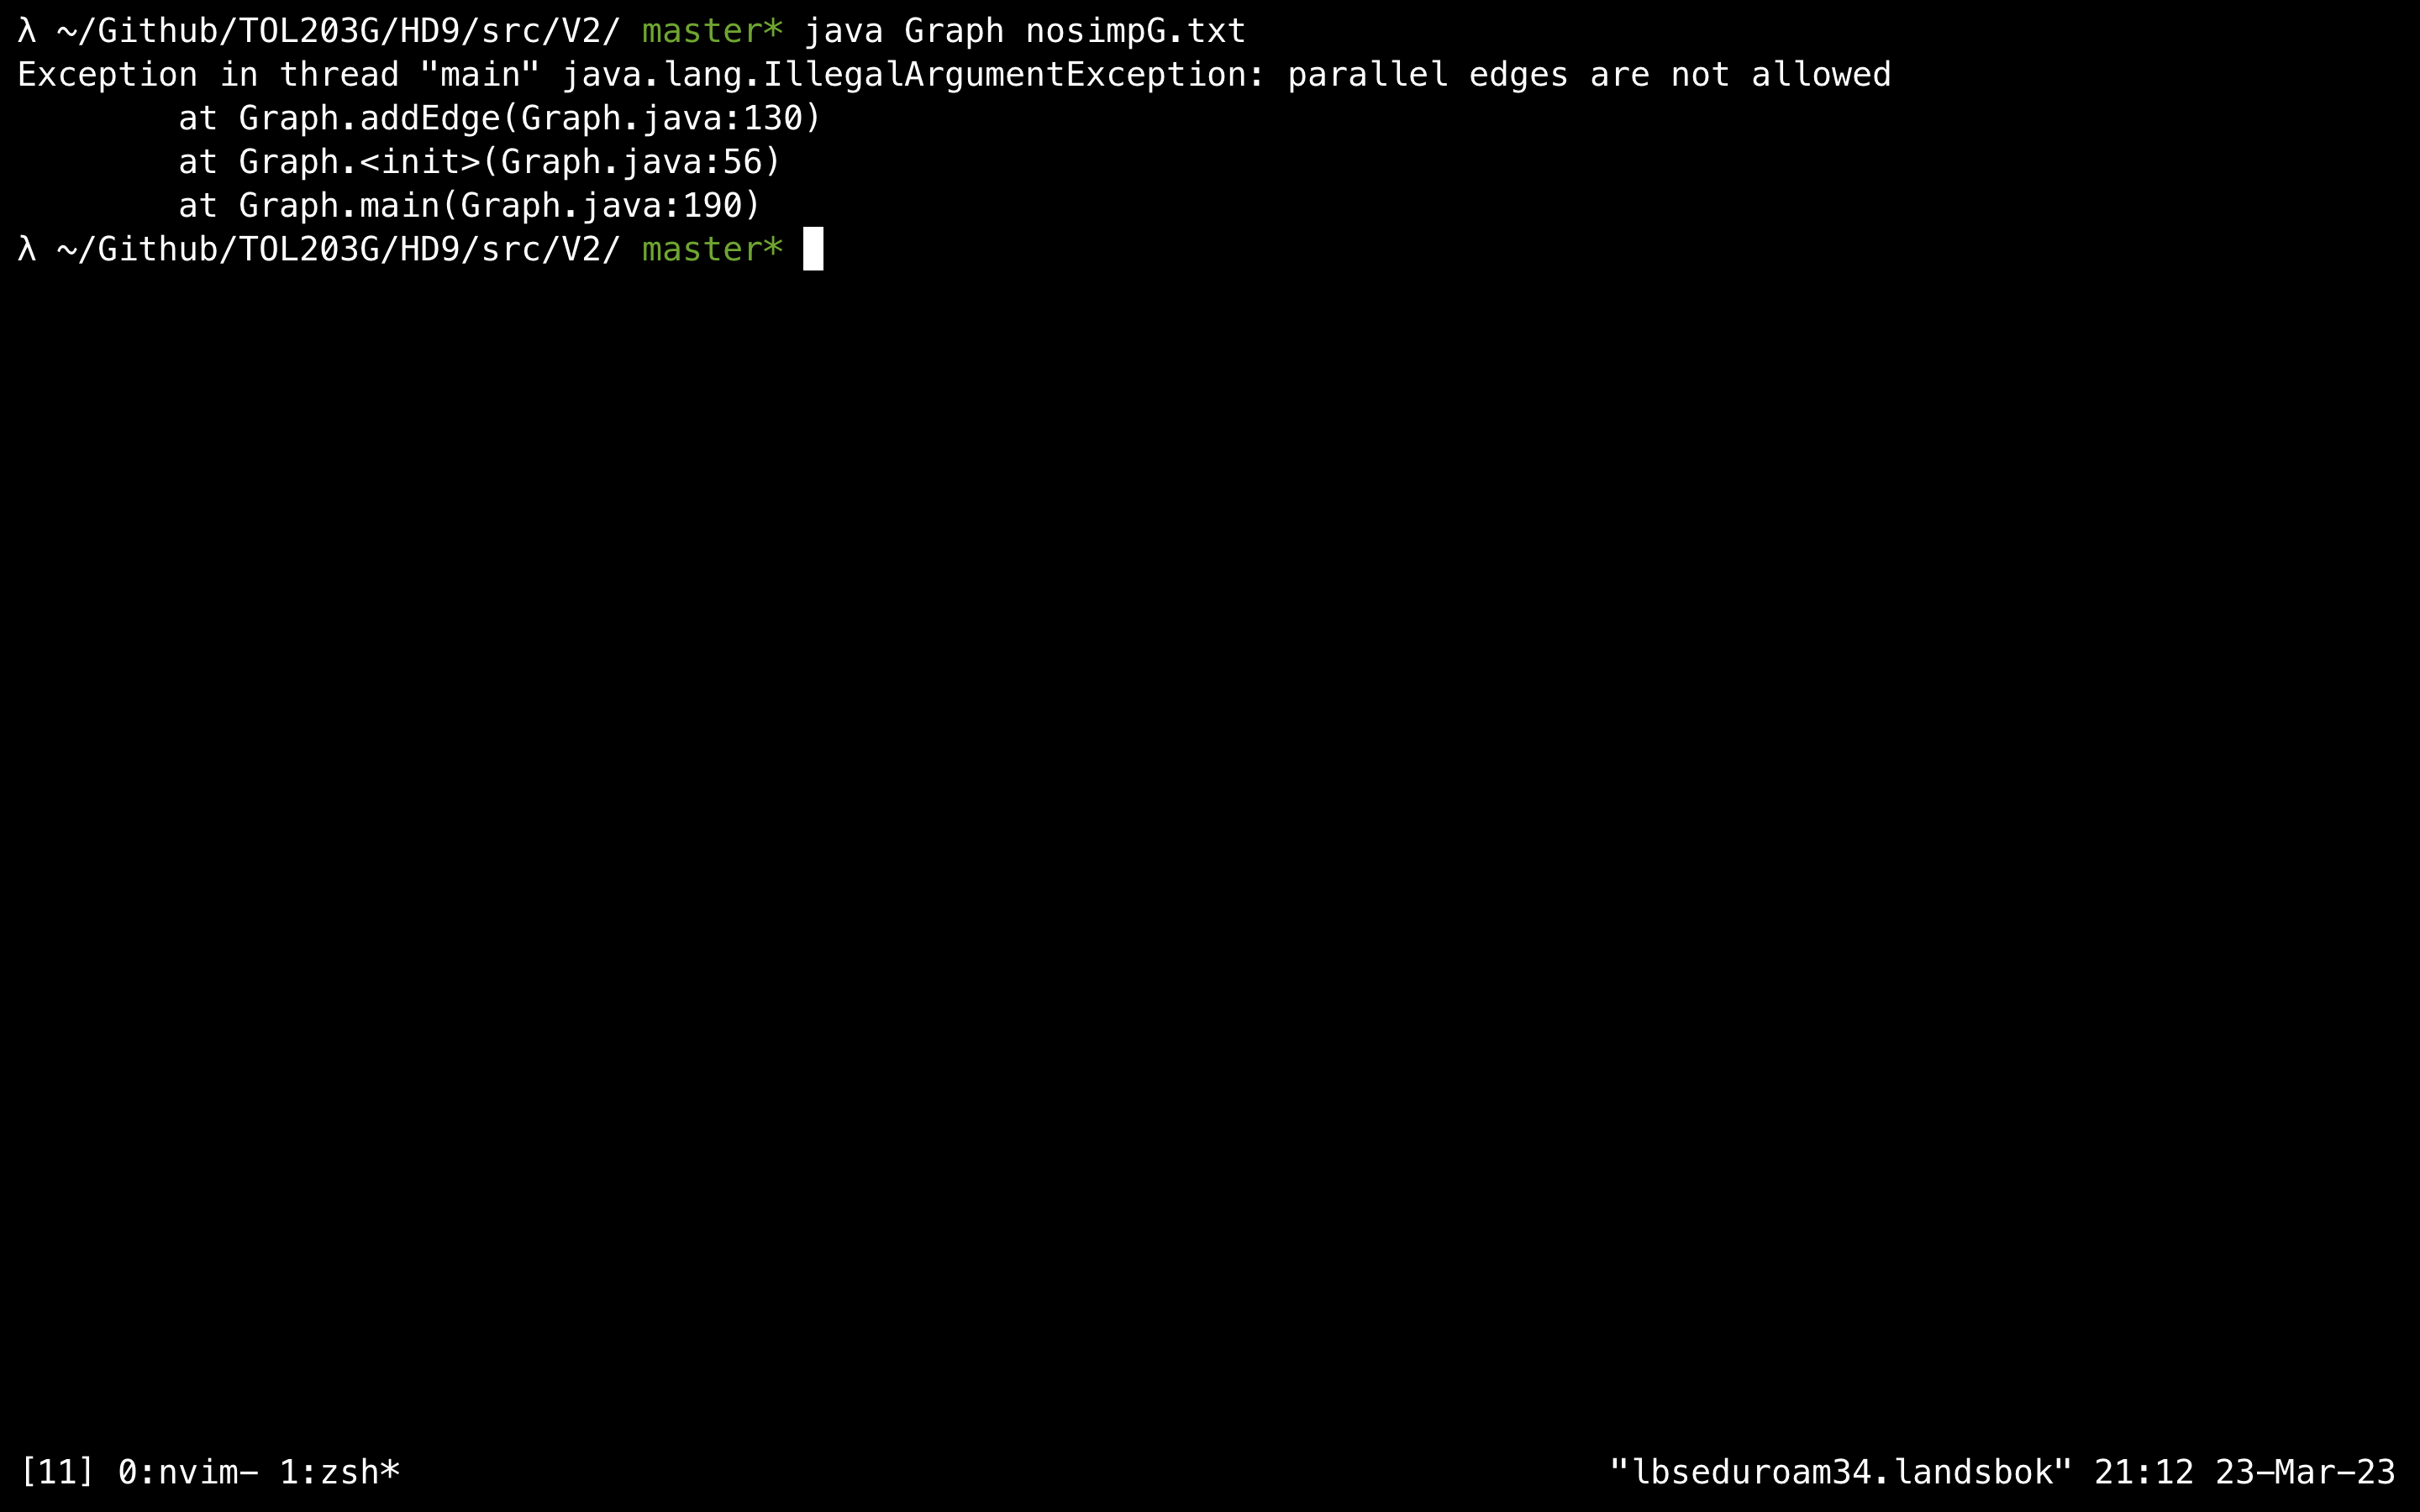
\includegraphics[width=\textwidth]{v2_keyrsla.png}
\caption{Keyrsla á nýrri útfærslu á \texttt{addEdge}}
\end{figure}
\newpage

\section*{Verkefni 3}
Sýnið röð hnúta sem grannfræðireikniritið sem sýnt var í fyrirlestri skilar þegar það er keyrt á eftirfarandi óhringuðu stefnuneti (DAG):
\begin{figure}[H]
    \centering
    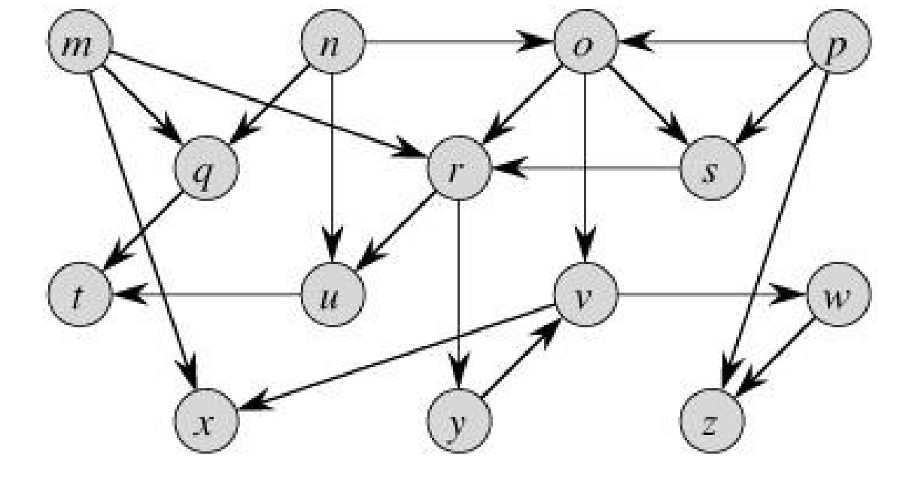
\includegraphics[width=0.7\textwidth]{v3_mynd.png}
    \end{figure}
\noindent
Gerið ráð fyrir að reikniritið skoði hnútana í stafrófsröð og að allir grannlistarnir séu í stafrófsröð.
\subsection*{Lausn}
Röðin sem kemur út úr reikniritinu er í öfugri eftirröð og er \texttt{y v w p z n o s m x r u q t}.
\newpage
\section*{Verkefni 4}
Skrifið aðferðina \texttt{noTriangle()} í klasann \texttt{Digraph}. Aðferðin finnur og skilar fjölda þrennda \texttt{u}, \texttt{v}, \texttt{w} þannig að \texttt{(u,v)} og \texttt{(v,w)} eru leggir í netinu \texttt{(u,w)} er ekki leggur. Þið megið nýa ykkur aðferðina \texttt{hasEdge} í æfingadæminu að ofan. Keyrið svo aðferðina á stefnunetið \texttt{tinyDG.txt} og sýnið úttakið (ætti að skila 37). Skilið líka aðferðinni sjálfri.

\subsection*{Lausn}
Útfærslan er fyrir neðan.
\begin{listing}[H]
    \centering
    \inputminted[linenos, breaklines, firstline=207, lastline=218]{java}{../src/V4/Digraph.java}
\end{listing}
\begin{figure}[H]
    \centering
    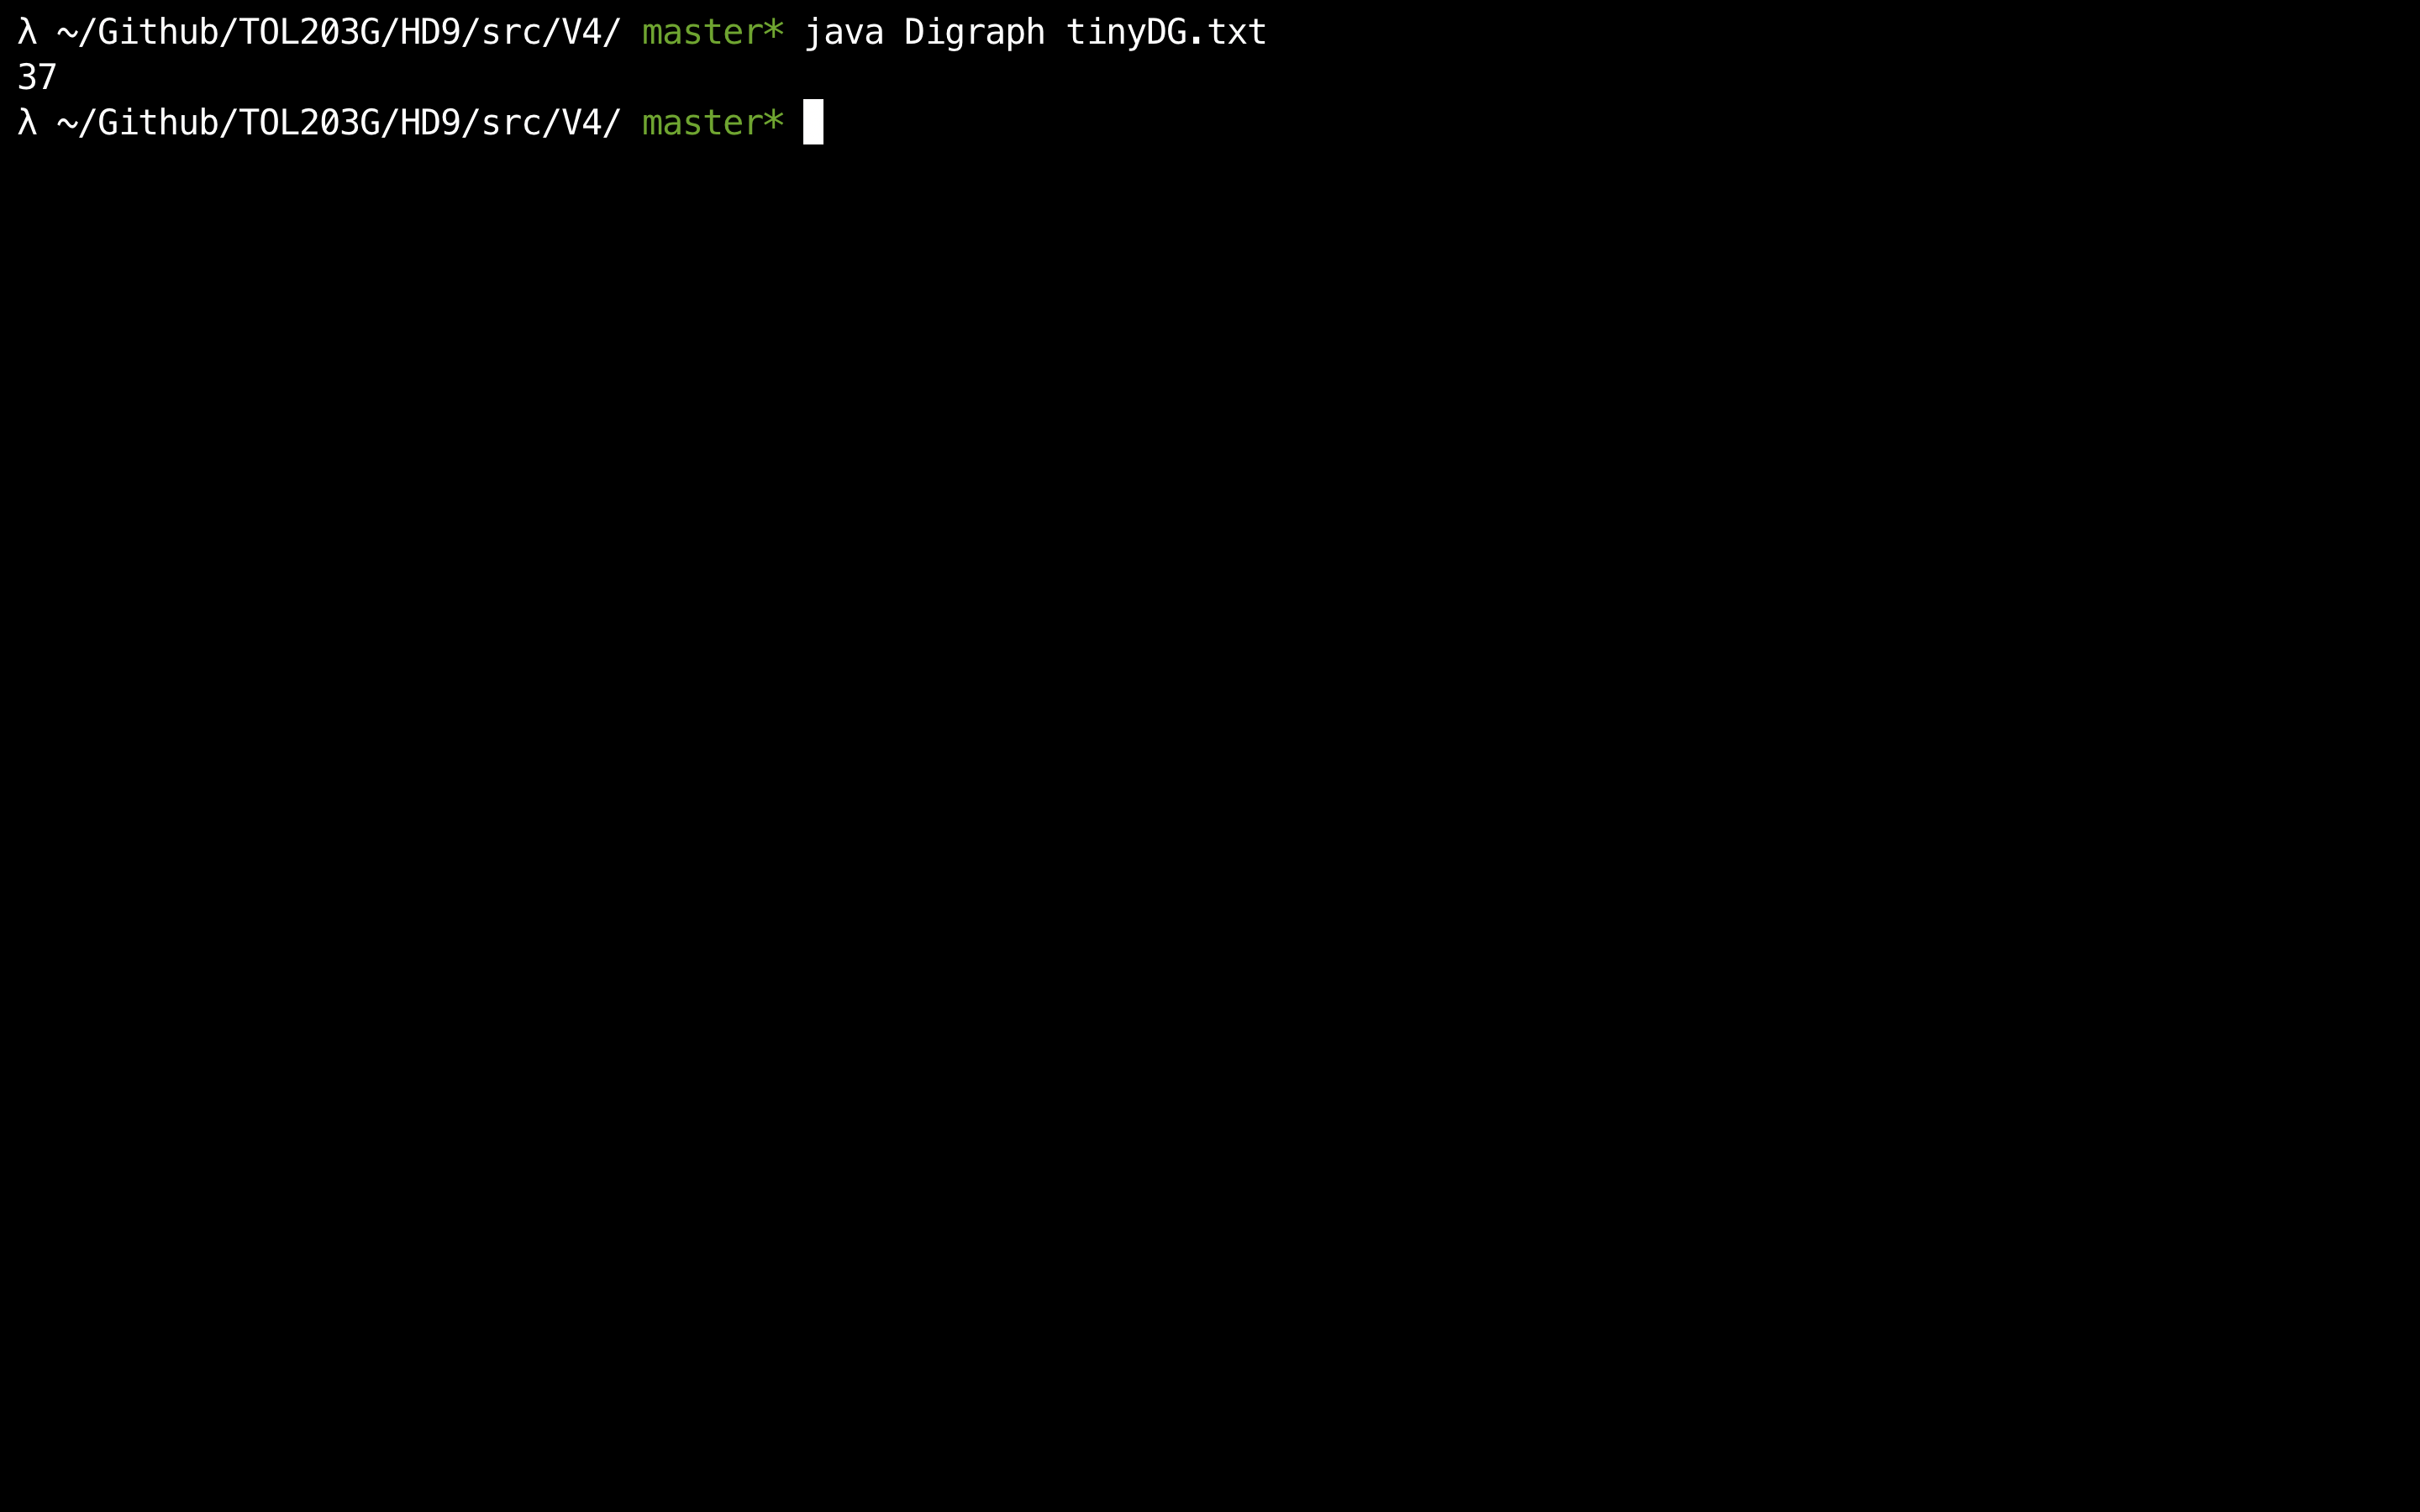
\includegraphics[width=0.8\textwidth]{v4_keyrsla.png}
\end{figure}

\end{document}
